\documentclass[tikz,12pt,border=2pt]{standalone}
\usepackage[T1]{fontenc}
\usetikzlibrary{arrows.meta,positioning,calc}
\definecolor{accent}{RGB}{31,84,140}
\definecolor{accentlight}{RGB}{200,214,232}
\begin{document}
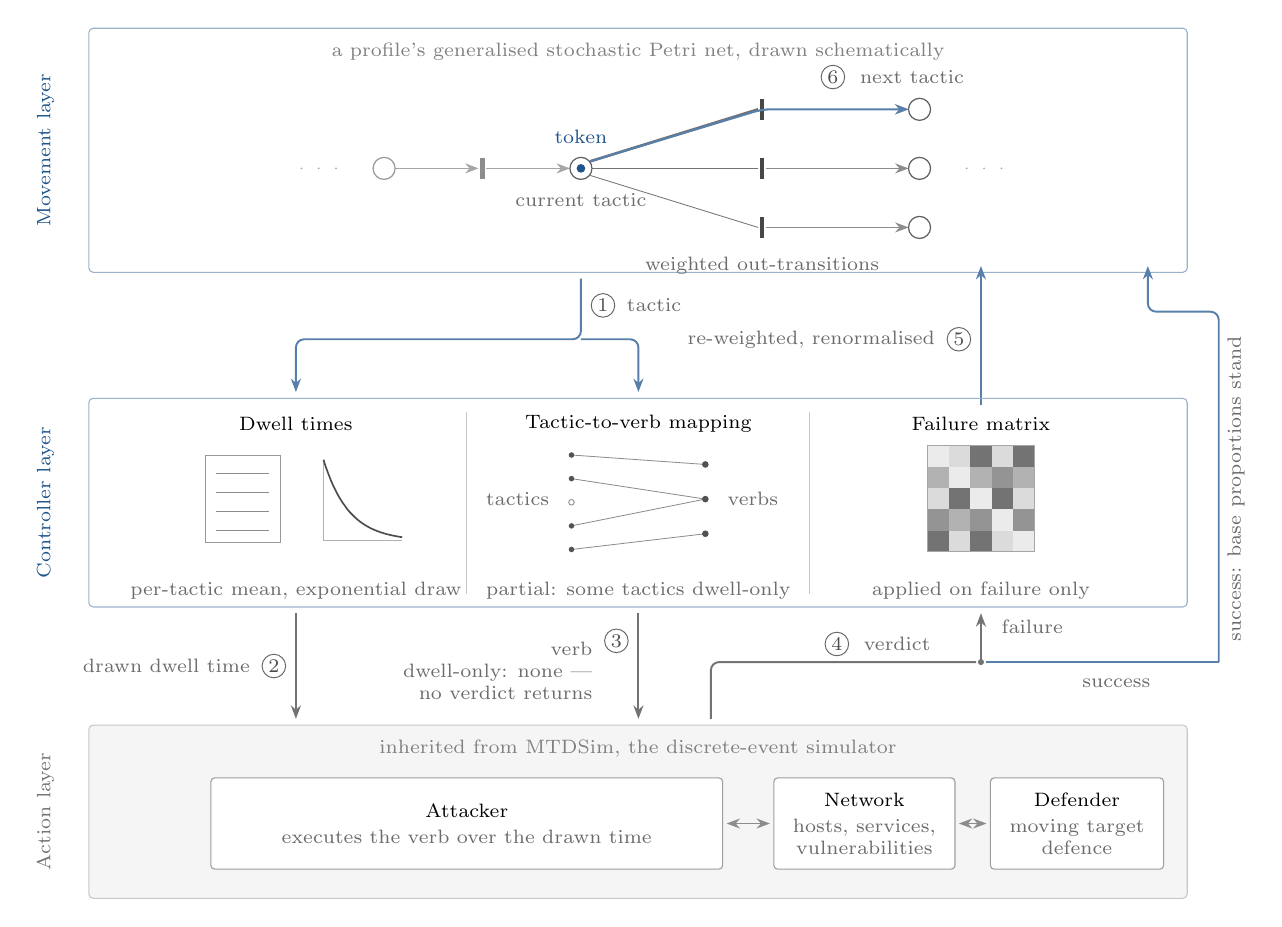
\begin{tikzpicture}[x=1cm,y=1cm,>={Stealth[length=1.7mm]},every node/.style={font=\scriptsize}]
\draw[draw=accent!45,line width=0.4pt,rounded corners=1.6pt] (0.850,-3.100) rectangle (14.800,0.000);
\node[rotate=90,anchor=center,font=\scriptsize,text=accent] at (0.300,-1.550) {Movement layer};
\node[anchor=north,font=\scriptsize,text=black!50] at (7.825,-0.060) {a profile's generalised stochastic Petri net, drawn schematically};
\draw[black!35,line width=0.4pt,->] (4.740,-1.780) -- (5.800,-1.780);
\draw[black!35,line width=0.4pt,->] (5.900,-1.780) -- (6.960,-1.780);
\draw[black!40,fill=white,line width=0.45pt] (4.600,-1.780) circle (0.140);
\fill[black!45] (5.820,-1.910) rectangle (5.880,-1.650);
\draw[black!55,line width=0.95pt] (7.219,-1.690) -- (9.350,-1.030);
\draw[black!55,line width=0.55pt] (7.219,-1.780) -- (9.350,-1.780);
\draw[black!55,line width=0.30pt] (7.219,-1.870) -- (9.350,-2.530);
\draw[black!45,line width=0.4pt,->] (9.450,-1.030) -- (11.260,-1.030);
\draw[black!45,line width=0.4pt,->] (9.450,-1.780) -- (11.260,-1.780);
\draw[black!45,line width=0.4pt,->] (9.450,-2.530) -- (11.260,-2.530);
\draw[black!62,fill=white,line width=0.45pt] (7.100,-1.780) circle (0.140);
\fill[black!72] (9.370,-1.160) rectangle (9.430,-0.900);
\fill[black!72] (9.370,-1.910) rectangle (9.430,-1.650);
\fill[black!72] (9.370,-2.660) rectangle (9.430,-2.400);
\draw[black!62,fill=white,line width=0.45pt] (11.400,-1.030) circle (0.140);
\draw[black!62,fill=white,line width=0.45pt] (11.400,-1.780) circle (0.140);
\draw[black!62,fill=white,line width=0.45pt] (11.400,-2.530) circle (0.140);
\fill[black!35] (3.550,-1.780) circle (0.35pt);
\fill[black!35] (3.770,-1.780) circle (0.35pt);
\fill[black!35] (3.990,-1.780) circle (0.35pt);
\fill[black!35] (12.000,-1.780) circle (0.35pt);
\fill[black!35] (12.220,-1.780) circle (0.35pt);
\fill[black!35] (12.440,-1.780) circle (0.35pt);
\fill[accent] (7.100,-1.780) circle (0.055);
\node[anchor=south,font=\scriptsize,text=accent] at (7.100,-1.590) {token};
\node[anchor=north,font=\scriptsize,text=black!58] at (7.100,-1.970) {current tactic};
\node[anchor=north,font=\scriptsize,text=black!58] at (9.400,-2.780) {weighted out-transitions};
\draw[->,accent!75,line width=0.75pt,rounded corners=3pt] (7.219,-1.690) -- (9.400,-1.030) -- (11.260,-1.030);
\node[circle,draw=black!60,text=black!70,inner sep=0.5pt,minimum size=8.5pt,line width=0.35pt,font=\scriptsize] at (10.300,-0.620) {6};
\node[anchor=west,font=\scriptsize,text=black!58] at (10.520,-0.620) {next tactic};
\draw[->,accent!75,line width=0.70pt,rounded corners=3pt] (7.100,-3.180) -- (7.100,-3.950) -- (3.480,-3.950) -- (3.480,-4.620);
\draw[->,accent!75,line width=0.70pt,rounded corners=3pt] (7.100,-3.950) -- (7.830,-3.950) -- (7.830,-4.620);
\node[circle,draw=black!60,text=black!70,inner sep=0.5pt,minimum size=8.5pt,line width=0.35pt,font=\scriptsize] at (7.380,-3.520) {1};
\node[anchor=west,font=\scriptsize,text=black!58] at (7.560,-3.520) {tactic};
\draw[->,accent!75,line width=0.70pt,rounded corners=3pt] (12.180,-4.780) -- (12.180,-3.020);
\node[circle,draw=black!60,text=black!70,inner sep=0.5pt,minimum size=8.5pt,line width=0.35pt,font=\scriptsize] at (11.900,-3.950) {5};
\node[anchor=east,font=\scriptsize,text=black!58] at (11.720,-3.950) {re-weighted, renormalised};
\draw[->,accent!75,line width=0.70pt,rounded corners=3pt] (15.200,-8.050) -- (15.200,-3.600) -- (14.300,-3.600) -- (14.300,-3.020);
\node[rotate=90,anchor=center,font=\scriptsize,text=black!58] at (15.420,-5.850) {success: base proportions stand};
\draw[draw=accent!45,line width=0.4pt,rounded corners=1.6pt] (0.850,-7.350) rectangle (14.800,-4.700);
\node[rotate=90,anchor=center,font=\scriptsize,text=accent] at (0.300,-6.025) {Controller layer};
\draw[black!22,line width=0.35pt] (5.650,-4.880) -- (5.650,-7.190);
\draw[black!22,line width=0.35pt] (10.000,-4.880) -- (10.000,-7.190);
\node[anchor=center,font=\scriptsize,text=black] at (3.480,-5.020) {Dwell times};
\draw[black!40,line width=0.35pt] (2.330,-6.530) rectangle (3.280,-5.420);
\draw[black!45,line width=0.3pt] (2.470,-5.660) -- (3.140,-5.660);
\draw[black!45,line width=0.3pt] (2.470,-5.900) -- (3.140,-5.900);
\draw[black!45,line width=0.3pt] (2.470,-6.140) -- (3.140,-6.140);
\draw[black!45,line width=0.3pt] (2.470,-6.380) -- (3.140,-6.380);
\draw[black!30,line width=0.3pt] (3.830,-5.480) -- (3.830,-6.510) -- (4.830,-6.510);
\draw[black!70,line width=0.6pt] (3.830,-5.480) -- (3.863,-5.581) -- (3.897,-5.672) -- (3.930,-5.755) -- (3.963,-5.829) -- (3.997,-5.896) -- (4.030,-5.956) -- (4.063,-6.010) -- (4.097,-6.059) -- (4.130,-6.104) -- (4.163,-6.144) -- (4.197,-6.179) -- (4.230,-6.212) -- (4.263,-6.241) -- (4.297,-6.268) -- (4.330,-6.291) -- (4.363,-6.313) -- (4.397,-6.332) -- (4.430,-6.350) -- (4.463,-6.365) -- (4.497,-6.380) -- (4.530,-6.392) -- (4.563,-6.404) -- (4.597,-6.414) -- (4.630,-6.424) -- (4.663,-6.432) -- (4.697,-6.440) -- (4.730,-6.447) -- (4.763,-6.453) -- (4.797,-6.459) -- (4.830,-6.464);
\node[anchor=north,font=\scriptsize,text=black!58,align=center] at (3.480,-6.910) {per-tactic mean, exponential draw};
\node[anchor=center,font=\scriptsize,text=black] at (7.830,-5.020) {Tactic-to-verb mapping};
\draw[black!45,line width=0.3pt] (6.980,-5.420) -- (8.680,-5.540);
\draw[black!45,line width=0.3pt] (6.980,-5.720) -- (8.680,-5.980);
\draw[black!45,line width=0.3pt] (6.980,-6.320) -- (8.680,-5.980);
\draw[black!45,line width=0.3pt] (6.980,-6.620) -- (8.680,-6.420);
\fill[black!68] (6.980,-5.420) circle (1.0pt);
\fill[black!68] (6.980,-5.720) circle (1.0pt);
\draw[black!42,line width=0.35pt] (6.980,-6.020) circle (1.0pt);
\fill[black!68] (6.980,-6.320) circle (1.0pt);
\fill[black!68] (6.980,-6.620) circle (1.0pt);
\fill[black!68] (8.680,-5.540) circle (1.2pt);
\fill[black!68] (8.680,-5.980) circle (1.2pt);
\fill[black!68] (8.680,-6.420) circle (1.2pt);
\node[anchor=east,font=\scriptsize,text=black!58] at (6.820,-5.975) {tactics};
\node[anchor=west,font=\scriptsize,text=black!58] at (8.840,-5.975) {verbs};
\node[anchor=north,font=\scriptsize,text=black!58,align=center] at (7.830,-6.910) {partial: some tactics dwell-only};
\node[anchor=center,font=\scriptsize,text=black] at (12.180,-5.020) {Failure matrix};
\fill[black!8] (11.505,-5.570) rectangle (11.775,-5.300);
\fill[black!14] (11.775,-5.570) rectangle (12.045,-5.300);
\fill[black!55] (12.045,-5.570) rectangle (12.315,-5.300);
\fill[black!14] (12.315,-5.570) rectangle (12.585,-5.300);
\fill[black!55] (12.585,-5.570) rectangle (12.855,-5.300);
\fill[black!30] (11.505,-5.840) rectangle (11.775,-5.570);
\fill[black!8] (11.775,-5.840) rectangle (12.045,-5.570);
\fill[black!30] (12.045,-5.840) rectangle (12.315,-5.570);
\fill[black!42] (12.315,-5.840) rectangle (12.585,-5.570);
\fill[black!30] (12.585,-5.840) rectangle (12.855,-5.570);
\fill[black!14] (11.505,-6.110) rectangle (11.775,-5.840);
\fill[black!55] (11.775,-6.110) rectangle (12.045,-5.840);
\fill[black!8] (12.045,-6.110) rectangle (12.315,-5.840);
\fill[black!55] (12.315,-6.110) rectangle (12.585,-5.840);
\fill[black!14] (12.585,-6.110) rectangle (12.855,-5.840);
\fill[black!42] (11.505,-6.380) rectangle (11.775,-6.110);
\fill[black!30] (11.775,-6.380) rectangle (12.045,-6.110);
\fill[black!42] (12.045,-6.380) rectangle (12.315,-6.110);
\fill[black!8] (12.315,-6.380) rectangle (12.585,-6.110);
\fill[black!42] (12.585,-6.380) rectangle (12.855,-6.110);
\fill[black!55] (11.505,-6.650) rectangle (11.775,-6.380);
\fill[black!14] (11.775,-6.650) rectangle (12.045,-6.380);
\fill[black!55] (12.045,-6.650) rectangle (12.315,-6.380);
\fill[black!14] (12.315,-6.650) rectangle (12.585,-6.380);
\fill[black!8] (12.585,-6.650) rectangle (12.855,-6.380);
\draw[black!35,line width=0.3pt] (11.505,-6.650) rectangle (12.855,-5.300);
\node[anchor=north,font=\scriptsize,text=black!58,align=center] at (12.180,-6.910) {applied on failure only};
\draw[->,black!55,line width=0.70pt,rounded corners=3pt] (3.480,-7.430) -- (3.480,-8.770);
\node[circle,draw=black!60,text=black!70,inner sep=0.5pt,minimum size=8.5pt,line width=0.35pt,font=\scriptsize] at (3.200,-8.100) {2};
\node[anchor=east,font=\scriptsize,text=black!58] at (3.020,-8.100) {drawn dwell time};
\draw[->,black!55,line width=0.70pt,rounded corners=3pt] (7.830,-7.430) -- (7.830,-8.770);
\node[circle,draw=black!60,text=black!70,inner sep=0.5pt,minimum size=8.5pt,line width=0.35pt,font=\scriptsize] at (7.550,-7.780) {3};
\node[anchor=east,align=right,font=\scriptsize,text=black!58] at (7.370,-8.160) {verb\\dwell-only: none ---\\no verdict returns};
\draw[-,black!55,line width=0.70pt,rounded corners=3pt] (8.750,-8.770) -- (8.750,-8.050) -- (12.120,-8.050);
\fill[black!55] (12.180,-8.050) circle (1.1pt);
\node[circle,draw=black!60,text=black!70,inner sep=0.5pt,minimum size=8.5pt,line width=0.35pt,font=\scriptsize] at (10.350,-7.820) {4};
\node[anchor=west,font=\scriptsize,text=black!58] at (10.570,-7.820) {verdict};
\draw[->,black!55,line width=0.70pt,rounded corners=3pt] (12.180,-8.050) -- (12.180,-7.430);
\node[anchor=west,font=\scriptsize,text=black!58] at (12.320,-7.600) {failure};
\draw[-,accent!75,line width=0.70pt,rounded corners=3pt] (12.240,-8.050) -- (15.200,-8.050);
\node[anchor=north,font=\scriptsize,text=black!58] at (13.900,-8.140) {success};
\draw[draw=black!22,line width=0.4pt,rounded corners=1.6pt,fill=black!4] (0.850,-11.050) rectangle (14.800,-8.850);
\node[rotate=90,anchor=center,font=\scriptsize,text=black!55] at (0.300,-9.950) {Action layer};
\node[anchor=north,font=\scriptsize,text=black!50] at (7.825,-8.910) {inherited from MTDSim, the discrete-event simulator};
\draw[black!38,fill=white,line width=0.4pt,rounded corners=1.4pt] (2.400,-10.680) rectangle (8.900,-9.520);
\node[font=\scriptsize,align=center,text width=6.34cm] at (5.650,-10.100) {Attacker\\[1.5pt]\color{black!58}executes the verb over the drawn time};
\draw[black!38,fill=white,line width=0.4pt,rounded corners=1.4pt] (9.550,-10.680) rectangle (11.850,-9.520);
\node[font=\scriptsize,align=center,text width=2.14cm] at (10.700,-10.100) {Network\\[1.5pt]\color{black!58}hosts, services,\\vulnerabilities};
\draw[black!38,fill=white,line width=0.4pt,rounded corners=1.4pt] (12.300,-10.680) rectangle (14.500,-9.520);
\node[font=\scriptsize,align=center,text width=2.04cm] at (13.400,-10.100) {Defender\\[1.5pt]\color{black!58}moving target\\defence};
\draw[<->,black!45,line width=0.5pt] (8.950,-10.100) -- (9.500,-10.100);
\draw[<->,black!45,line width=0.5pt] (11.900,-10.100) -- (12.250,-10.100);
\end{tikzpicture}
\end{document}
